\documentclass[oneside,4papera,12pt]{report}
% Page de garde, dedicace, remerciements, resumés non numérotée

%------------------------------Zone 1-------------------------
\usepackage{tabularx}
\usepackage{float}
\usepackage[left=2cm,right=2cm,top=3cm,bottom=3cm]{geometry}

%% DEBUT MOL
\usepackage[explicit]{titlesec}
\usepackage{tikz}
\usepackage{titletoc}
\usepackage{xpatch}
\definecolor{myblue}{RGB}{0,0,0}

\newcommand\DoPToC{%
	\startcontents[chapters]
	\printcontents[chapters]{}{1}{\noindent{\color{myblue}\rule{\textwidth}{1.5pt}}\par\medskip}%
}

\usepackage{fancyhdr}
\setlength{\headheight}{9pt}
\pagestyle{fancy}
%\usepackage{lastpage}
\renewcommand\headrulewidth{0.5pt}
\fancyhead[L]{\scshape\leftmark\hspace{0,3cm}}
\renewcommand\footrulewidth{0.5pt}
\fancyfoot[C]{
	\textbf{
		\begin{tikzpicture}[baseline={([yshift=-.05ex]current bounding box.center)}]
			\node[fill=black,circle,text=white] {{{\thepage}
			}};
		\end{tikzpicture}
	}
}
\fancyhead[R]{2020-2021}


\usepackage{enumitem}
\usepackage{amssymb}

\usepackage{hyperref}
\hypersetup{colorlinks,%
	citecolor=black,%
	filecolor=black,%
	linkcolor=black,%
	urlcolor=black
}

\usepackage{tikz}
\usetikzlibrary{shadows.blur}
\usepackage{titletoc}

\usepackage[]{titlesec} 
\definecolor{yourcolor}{HTML}{000000}
\definecolor{noir}{HTML}{000000}

\usepackage{nomencl} 
\makenomenclature 
\renewcommand{\nomname}{Liste des abréviations, des sigles}% Pour redéfinir le titre De cette liste


%%% FINNNNNN MOL
\usepackage{fancyhdr}
\usepackage[utf8]{inputenc}

\usepackage[T1]{fontenc}
\usepackage[french]{babel}
\usepackage{graphicx}
\usepackage{refstyle}
\usepackage{caption}
\usepackage{adjustbox}

\usepackage{array,multirow,makecell}
\usepackage{tabularx}
\renewcommand{\tabularxcolumn}{m}



\setcellgapes{1pt}
%\makegapedcells
\newcolumntype{R}[1]{>{\raggedleft\arraybackslash }b{#1}}
\newcolumntype{L}[1]{>{\raggedright\arraybackslash }b{#1}}
\newcolumntype{C}[1]{>{\centering\arraybackslash }b{#1}}

%------------------------------Fin Zone 1---------------------------

\begin{document}
	%------------Zone 2: début des page non numérotées-------------------------
	\begin{titlepage}
	\begin{center}
		{\bf \textsc{REPUBLIQUE DE COTE D'IVOIRE}\\
			\vspace*{2mm}		
			\textbf{\textsc{Union-Discipline-Travail}} \\
		}
		\hrulefill \\
		\textbf{\textsc{Minist\`ere de l\textquoteright Enseignement Sup\'erieur et de la Recherche Scientifique}} \\
		\hrulefill \\		
		\textbf{\textsc\LARGE {UNIVERSITE NANGUI ABROGOUA}}
		\\
		\hrulefill \\		
		\vspace*{2mm}		
		\textbf{\textsc\LARGE {Unit\'e Fondamentale de Recherche des Sciences Fondamentales et Appliqu\'ees}}\\[0.1cm]
		\vspace*{3mm}
		\textbf{\textsc{2020-2021}}
	\end{center}
	\begin{figure}[!h]
		\begin{minipage}[t]{.1\linewidth}
			\begin{flushleft}
				\begin{center}
					
\includegraphics[scale=0.5]{images/una}
				\end{center}
			\end{flushleft}
		\end{minipage}
		\hfill
		\begin{minipage}[t]{.1\linewidth}
			\begin{flushright}
				\begin{center}
					
\includegraphics[scale=0.5]{images/sfa}
				\end{center}    		
			\end{flushright}
		\end{minipage}
	\end{figure}
	\begin{center}
		\textbf{\textsc{M\'emoire pour obtention du diplôme de master}} 
		\\[0.1cm]
		Mention : \textbf{\textsc{informatique}}\\[0.05cm]
		Spécialité : \textbf{\textsc{génie informatique}}\\[0.05cm]
		
		\normalsize
		\vspace{0.005cm}
		\Huge\textbf{\textsc{Th\`eme}}\\
		\noindent\rule{\textwidth}{0.9mm}
		\Large{{\textbf{\textcolor{red}{\textsc{Conception d\textquoteright une application de transfert d'unité de communication pour l'entreprise ONEMART}}}}}
		\noindent\rule{\textwidth}{0.9mm}
	\end{center}
	\begin{center}
		\textbf{Présenté par : } \\
		\begin{center}
			\textsc{TUO ADAMA}
		\end{center}
		\vspace*{0.5mm}
		\textbf{Date de soutenance : } xx octobre 2021  
	\end{center}
	\vspace*{2mm}
	% Author and supervisor
	\begin{minipage}{0.5\textwidth}
		\begin{flushleft} \large
			\textbf{Composition du jury : } 
			\begin{itemize}[leftmargin=* ,parsep=0cm,itemsep=0.2cm,topsep=0.2cm]
				\item{\textbf{Pr\'esident : }}
				\item {\textbf{Membre : }}
				\item {\textbf{Membre : }}
				\item {\textbf{Membre : }}
			\end{itemize}  
		\end{flushleft}
	\end{minipage}
	\begin{minipage}{0.5\textwidth}
		\begin{flushright} \large
			\textbf{Encadreur : } \\ Dr ZEZE DJEDJE SYLVAIN, Maitre-Assistant UNA
		\end{flushright}
	\end{minipage}
	
\end{titlepage}
	\chapter*{Remerciements}
	\thispagestyle{empty}
	
%	Je voudrais tout d’abord adresser toute ma reconnaissance à mon encadreur Dr Zézé Sylvain pour sa disponibilité et surtout ses judicieux conseils, qui ont contribué à alimenter ma réflexion tout au long de ce projet.
	
	Tout d'abord ce travail ne serait pas aussi riche et n'aurait pas pu voir le jour sans l'aide de l'encadrement de \textbf{Dr Zézé Sylvain}, je vous remercie pour la qualité exceptionnelle de votre encadrement, votre rigueur et surtout votre disponibilité durant la préparation de ce mémoire.\\
	
	
	Mon remerciement s'adresse à \textbf{Dr Tchimou N'Takpé} pour ses encouragements et ses précieux conseils.
	
	J’adresse mes sincères remerciements à tous les professeurs, intervenants et toutes les personnes qui par leurs paroles, leurs écrits, leurs conseils et leurs critiques ont guidé mes réflexions tout au long de la rédaction de ce mémoire.\\
	
	Je remercie mes très chers parents, \textbf{Kone Naminata} et \textbf{Tuo Zahana}, qui ont toujours été là pour moi. Je remercie surtout mon oncle \textbf{Kone Souleymane} pour ses encouragements sans fin tout au long de mon parcours scolaire.\\
	
	À tous ces intervenants, je présente mes remerciements, mon respect et ma gratitude.
	\chapter*{Dédicaces}
	\thispagestyle{empty}
	
	A mes très chers parents \textbf{Tuo Zahana} et \textbf{Kone Naminata} qui ont toujours été là pour moi, qui m'ont soutenu et encouragé durant toutes ces années d'études. J'espère qu'ils trouveront dans ce travail toute ma reconnaissance et tout mon
	amour.\\
	
	A mon cher frère \textbf{Tuo Kolo} et à mes sœurs : \textbf{Tuo Yoh abi}, \textbf{Yire Fatoumata} et \textbf{Barah Ramatou}.\\
	
	
	A mes meilleurs amies
	
	\begin{center}
		Je dédie ce mémoire.
	\end{center}
	\chapter*{Résumé}
	\thispagestyle{empty}
	
%	Faisant face à un système obsolète basé sur une architecture complexe, l'entreprise ONEMART retrouvait sa productivité altérée par le fait de la non-automatisation des tâches qu'elle effectuait.\\
%	C'est dans cette optique que s'est déroulé le stage de notre mémoire de Master. En effet tout au long de ce stage nous avons eu à mettre une application optimisée et maintenable répondant aux exigence de l'entreprise.\\
%	Afin carder le développement de notre application et la mise en place d'une architecture solide, nous avons fait appel à des méthodes de conceptions impeccables dans le but de mener à bien ce projet.
	
	Faisant face à un système obsolète basé sur une architecture complexe, l'entreprise ONEMART retrouvait sa productivité altérée par le fait de la non-automatisation des tâches qu'elle effectuait.\\
	C'est dans cette optique que s'est déroulée le stage de notre mémoire de Master. En effet tout au long de ce stage nous avons eu à mettre une application Web de transferts et recouvrement d'argent à une plage de client ( aussi appelé intermède) suivant un mode de paiement donnée (Crédit, comptant, bancaire, etc ...). Une fois l'opération (transfert ou recouvrement) effectuée, grâce à l'interopérabilité offerte par l'application, un système externe (nous avons aussi appelé validateur) récupère les informations de l'opération et la valide grâce à une syntaxe USSD.\\
	Ainsi Afin de cadrer le développement de notre application et de répondre aux exigences de l'entreprise, nous avons élaboré un plan de conception grâce aux différents diagrammes UML. Vu les fonctionnalités offertes par l'application, elle a été développée en utilisant le framework \textbf{Laravel} et d'autres outils de développement (le système de gestion de base de donnée relationnelle \textbf{MySQL}, une bibliothèque JavaScript \textbf{AlpineJs}, etc...) pour faciliter le développement de l'application tout en assurant une bonne sécurité de celle-ci.\\
	
	\textbf{Mots clés}: Interopérabilité, Productivité, Transferts, Recouvrements, Rechargements
	
%	Faire des transfert à un plage d'intermède,
%	Intermède fait le transfert suivant un mode de paiement
%	A l'aide de quels outils ?
%	Comment avons nous 	réglé ce problème ?
%	
	\chapter*{Abstract}
\thispagestyle{empty}
	Faced with an obsolete system based on a complex architecture, ONEMART
	found its productivity altered by the fact of the non-automation of the tasks it was carrying out.
	It is in this perspective that the internship of our Master's thesis took place. In fact, throughout this
	throughout this training course we had to put a Web application of transfers and recovery of ar-
	gent to a range of customer (also called intermediary) according to a given method of payment (Credit,
	cash, bank, etc ...). Once the operation (transfer or recovery) is done, thanks to the
	interoperability provided by the application, an external system (also called validator)
	retrieves the information of the operation and validates it thanks to a USSD syntax.
	Thus, in order to frame the development of our application and to meet the requirements of the company, we
	In order to frame the development of our application and to meet the requirements of the company, we have elaborated a design plan thanks to the various UML diagrams. Given the
	functionalities offered by the application, it was developed using the Laravel framework and other
	other development tools (the relational database management system MySQL ,
	a JavaScript library AlpineJs, etc. ...) to facilitate the development of the application while
	while ensuring a good security of this one.\\
	
	Key words : Interoperability, Productivity, Transfers, Recoveries, Reloads
		\addcontentsline{toc}{chapter}{Resumé}
	%------------Fin Zone 2: fin des page non numérotées------------------------
	
	%------------Zone 3:début entêtes et prieds de page-------------------------------
	\pagestyle{fancy}
	\fancyhead[L]{}
	
	\fancyfoot[L]{TUO Adama}
	\fancyfoot[R]{\thepage}
	\fancyfoot[C]{}
	%
	%\fancyfoot[R]{\ch}
	
	%------------Fin Zone 3: fin des entêtes et prieds de page ---------------
	
	%------------Zone 4: début de la numérotation avec les chiffres romains-----------------
	
	\tableofcontents
		\pagenumbering{roman}
		\setcounter{page}{1}
	\listoftables
	\addcontentsline{toc}{chapter}{Liste des tableaux}
	\listoffigures
	\addcontentsline{toc}{chapter}{Table des figures}
	
	\chapter*{Liste des abréviations}


\begin{flushleft}
	\textbf{MERISE}   \textbf{M}éthode d'\textbf{É}tude et de \textbf{I}nformatique pour les \textbf{S}ystèmes d'\textbf{E}ntreprise\\
\end{flushleft}

\begin{flushleft}
	\textbf{UML}  \textbf{U}nified \textbf{M}odeling \textbf{L}anguage
\end{flushleft}

\begin{flushleft}
	\textbf{VPN}  \textbf{V}irtual \textbf{P}rivate \textbf{N}etwork
\end{flushleft}

\begin{flushleft}
	\textbf{PC}  \textbf{P}ersonnal \textbf{C}omputer
\end{flushleft}

\begin{flushleft}
	\textbf{API}  \textbf{A}pplication \textbf{P}rogramming \textbf{I}nterface
\end{flushleft}

\begin{flushleft}
	\textbf{HTML}  \textbf{H}yper \textbf{T}ext \textbf{M}arkup \textbf{L}anguage
\end{flushleft}

\begin{flushleft}
	\textbf{CSS}  \textbf{C}ascading \textbf{S}tyle \textbf{S}heets
\end{flushleft}

\begin{flushleft}
	\textbf{MVC}  \textbf{M}odel \textbf{V}iew \textbf{C}ontroller
\end{flushleft}
		\addcontentsline{toc}{chapter}{Liste des abréviations}
	
	%------------Fin Zone 4: fin de la numérotation avec les chiffres romains---
	
	%-----------------Zone 5: début de la numérotation avec les chiffres arabs-----------
	
	\chapter*{Introduction générale}

Depuis longtemps, La technologie n'a cessé d'augmenter la productivité de milliers d'entreprises presque dans tous les secteurs d'activités.\\
Le passage de la mécanique aux domaines de l'informatique, de l'électronique de la domotique a révolutionné la vie journalière de l'être humain.
Aujourd'hui, vu l'intérêt croissant de vouloir gagner en temps, d'automatiser les tâches répétitives, cela a poussé petites, moyennes et grandes entreprises à chercher des solutions informatiques capables de répondre à leurs besoins.\\
C'est dans ce cadre s'inscrit notre projet de fin d'études qui consiste à réaliser une application de transfert et de recouvrement pour une entreprise appelée \textbf{ONEMART}.
Il y'a quelques années de cela, l'entreprise ONEMART faisait face à une application legacy qui etait difficile à maintenir. Du coup elle retrouvait une baisse au niveau de sa productivité par le fait de la non maintenabilité des différents système informatique dont elle disposait.\\
En effet, c'est face à ces différents problème que nous avons l'opportunité le contexte de notre stage de master. Ainsi notre objectif a été de partir d'une application legacy et développer une nouvelle application qui pourra s'adapter dans le temps et pourra apporter un gain de temps de considérable à l'entreprise.\\

Ainsi pour bien cadrer l'étude de ce stage, notre travail se présentera comme suite :\\
\begin{itemize}
	\item En premier lieu nous allons présenter l'entreprise \textbf{ONEMART} et le cadre dans lequel se situera le projet.
	\item En second lieu nous allons faire la présentation des différentes phases de conception et l'étude technique du projet.
	\item Enfin nous présenterons l'application grâce aux différentes captures d'écran accompagnées de quelques détails.
\end{itemize}
		\addcontentsline{toc}{chapter}{Introduction générale}
		\pagenumbering{arabic}
		\setcounter{page}{1}
	\chapter{CADRE GÉNÉRAL}
\section{Introduction}
	Dans ce chapitre nous allons présenter ONEMART, la société pour laquelle nous avons effectué notre application de fin de cycle. Ensuite la présentation du cadre du projet permettra de mieux comprendre le problème étudié et présenter le principe de fonctionnement de l'application mise en place.
	Enfin, ce chapitre présentera la solution retenue qui sera détaillée plus loin dans ce mémoire.
\section{Présentation de l'entreprise}
	ONEMART est une société expérimentée dans la commercialisation des produits et services de la téléphonie mobile sur le marché national et bénéficiant d’un personnel hautement qualifié. Onemart dispose d’un réseau propre avec plusieurs points de vente mais aussi d’un portefeuille clientèle conséquent. Depuis janvier 2010, elle est le distributeur exclusif (franchisé) d’atlantique télécom CI, société de droit ivoirien propriétaire d’un réseau de radiotéléphonie cellulaire  exploité sous la marque Moov.\\
	
	ONEMART assure ainsi l’exclusivité de la distribution des produits et des services de Moov (Kits, recharges physiques et électroniques, portables et autres services après vente) dans les zones géographiques suivantes: Yopougon, Dabou, Sikensi, Tiassale, N’douci, Jacqueville, Grand-lahou, N’zianoua,.\\
	
	
\section{Cadre du projet} % Developpement web %
	Dans le cadre de notre mémoire nous nous sommes concentrés sur une des branches de l'entreprise qui est le rechargement des clients qui sont aussi appelés intermèdes.
\subsection{Problématique}
		Dans les années antérieures, l'entreprise ONEMART disposait d'une application VB déjà compilée avec toutes les plages de numéros dont elle disposait. Ainsi lors du passage des numérotations à dix chiffres, l'entreprise faisait face à un très gros problème qui était de mettre à jour les numéros des intermèdes vu que le code source de l'application n'était plus disponible.
		\paragraph{}A son siège, l'entreprise disposait d'un PC central câblé en local avec un téléphone d'ancienne génération(Sony Ericsson) équipé d'une puce \textbf{emaster} qui récupérait par câble les opérations effectuées (Recouvrement et transfert) sur le PC pour les valider. Ainsi, pour faire des rechargements et transferts depuis un point de vente distant, l'on devait se connecter par VPN (Virtual Private Network) pour avoir accès au PC central. En effet, puisque le VPN fait transiter la connexion de l'utilisateur par un serveur distant, ce qui rajoute une étape intermédiaire lors de la transmission des informations. Ainsi l'on fait face à un débit de transmission moins stable.
		\paragraph{}Aussi sur le point sécuritaire, il est important de noter que les opérations se faisaient manuellement sachant bien que les montants de transfert étaient très élevés ce qui pouvait être très problématique du moment où l'on peut être exposé aux problèmes suivants: Se tromper sur le montant de transfert, transférer l'argent d'un intermède	à un autre.\\
		
\subsection{Objectifs du projet}
	Face aux problèmes cités ci-dessus, notre application aura pour objectifs de :
	\begin{itemize}
		
		\item Mettre en place une application WEB car en plus d’être accessible sur toutes les plateforme (peu importe le système d'exploitation de l'utilisateur), elle est simple et nécessite aucune installation.\\
		
		
		
		\item Que de passer par VPN (Virtual Private Network) pour avoir accès au PC central, l’application sera accessible peu importe la situation géographique de l'utilisateur.\\
		
		\item Fournir une interopérabilité entre l'application et d'autre système externe. C'est à dire rendre accessible par API (Application Programming Interface) les informations de transfert et recouvrement après chaque opération pour qu'un autre système puissent les récupérer et les valider par \textbf{USSD}.\\
		
		\item Offrir plusieurs modes de paiement aux intermèdes lors des transferts: comptant, crédit, bancaire, etc...
		
		\item Fournir une facture après chaque opération.
		
		
	\end{itemize}
\subsection{Élaboration du cahier des charges}
	
	Dans cette section, nous allons définir les différentes charges que notre application devra respecter lors de la conception.
	L'application aura pour charge :
	\begin{itemize}
		\item Créer un point d'entrée par lequel les données seront accessible par un autre système externe.\\
		\item Persister les messages de transferts et recouvrement\\
		\item Sauvegarder les historiques de transfert.\\
		\item Gérer la liste des intermèdes en ayant la possibilité de la modifier, ajouter et supprimer sans oublier de leur attribuer des numéros.\\
		\item Gestion du mode de paiement (paiement par carte bancaire, crédit ou comptant).\\
		\item Élaboration d'une facture après chaque opération avec la possibilité de la télécharger.\\
		\item Gérer l'état des opérations:\\
			\begin{itemize}
				\item[$\bullet$]  état initié : Lorsque l'opération vient d'être effectuée.\\
				\item[$\bullet$] cours d'exécution: Lorsque l'application mobile récupère le message d'opération pour la valider.\\
				\item[$\bullet$] exécuté: Lorsque l'opération est effectuée par l'application.\\
				\item[$\bullet$] annulé: Lorsque le l'opération est annulée.
			\end{itemize}
	\end{itemize}

\subsection{Planification de l'application}
	Que l’on soit chef d’équipe ou responsable de sa propre activité, bien planifier ses projets est essentiel pour être efficace. Cela permet d’organiser son temps dépendamment du travail à réaliser, et de garantir son efficacité sur le long terme. Ainsi la planification d'une application passe par plusieurs étapes(qui peux dépendre d'une application à une autre ) telle que:\\
	
	\begin{itemize}
		\item Étape n° 1 : \textbf{analyse fonctionnelle et définition des objectifs} : Cette partie consistera à rechercher et à caractériser les fonctions offertes par notre application pour satisfaire les différents besoins du client.\\
		\item Étape n° 2 : \textbf{conception détaillée}: La phase de conception détaillée donne lieu à la rédaction du cahier des charges opérationnel. C'est elle qui précisera les différents éléments de dimensionnement du projet.\cite{planification} C'est aussi dans cette étape qu'entre la modélisation du système avec des méthodes de modélisations comme MERISE.\\
		\item Étape n° 3 : \textbf{développement du projet}: C'est dans cette  partie qu'entre en jeu la partie technique de l'application. Cette étapes exige la maîtrise d'au moins un langage de programmation.\\
		\item Étape n° 4 : \textbf{Phase de tests}:
		%Tests unitaires, tests d'integration ,tests de validation%
		C'est l'ensemble des tests(tests unitaires, tests d'intégration et tests de validation) qui permettront de retrouver les erreurs moins évidentes qui n'ont pas été détectées pendant la phase de développement.\\
		\item Étape n° 5 : \textbf{recette}: Permet de s'assurer que l'application développée correspond bien aux exigences fixées par le client.\\
		\item Étape n° 6 : \textbf{mise en production}: Déploiement de l'application.\\
		\item Étape n° 7 : \textbf{maintenance}: On entend par maintenance, l'ensemble des modifications mises en place après la mise en œuvre de l'application en production afin de corriger les bogues, améliorer les performances ou encore l'adapter à une modification de son environnement.\cite{planification}
	\end{itemize}
	
\section{Conclusion}
	Dans ce chapitre nous avons présenté \textbf{ONEMART} ainsi que ses différentes activités. Nous avons cadré le projet sur lequel tient notre mémoire en définissant la problématique, les objectifs, le cahier des charges et enfin le plan sur lequel se déroulera le développement de l'application. Le prochain chapitre sera dédié à la conception et à l'analyse des besoins de l'entreprise.
	\chapter{CONCEPTION ET ÉTUDE TECHNIQUE}
	\section{Conception}
	
	Face à leur grandeur, le développement des systèmes d'information devient de plus en plus complexe. Prévoir les fonctionnalités du système devient alors moins évidentes, c'est ainsi qu'entre en jeu la phase de conception. La phase de conception nécessite des outils permettant de mettre en place un modèle sur lequel on va s'appuyer pour réaliser notre application.
	

	\section{Présentation de UML}
			UML est un langage de modélisation très complet, qui couvre de nombreux aspects du développement des logiciels, comme les exigences, l’architecture, les structures et les comportements.\\
			
			Depuis sa normalisation, en 1997, UML a fortement évolué, passant d’un langage peu	formel, principalement destiné à la documentation, à un langage suffisamment précis pour que des applications puissent être générées à partir des modèles. Cette évolution	vers une plus grande précision a cependant créé une césure entre les tenants du « tout modèle », qui demandent toujours plus de formalisme, et les développeurs, qui apprécient UML pour sa capacité à capturer en quelques dessins les grandes lignes d’une
			application.
		\subsection{Principaux diagrammes UML}
			UML dispose à sa version actuelle (2.5.1) de treize diagrammes qui sont regroupés en deux grandes catégories tels que les diagrammes structurels et les diagrammes de comportements.
		\subsubsection{Diagramme structurels}
			Ces diagrammes permettent de visualiser, spécifier, construire et documenter l'aspect statique ou structurel du système d'information. Voici quelques diagrammes utilisés couramment:\\
			\begin{itemize}
				\item Diagramme de classe: Ce diagramme représente la description statique du système en intégrant dans chaque classe la partie dédiée aux données et celle consacrée aux traitements. C’est le diagramme pivot de l’ensemble de la modélisation d’un système.\cite{definition_diagramme_classe}\\
				
				\item Diagramme de composant: Ce diagramme représente
				les différents constituants du logiciel au niveau de l’implémentation d’n système.\cite{definition_diagramme_composant}\\
				
				\item Diagramme de paquetage: Ce diagramme donne une
				vue d’ensemble du système structuré en paquetage. Chaque paquetage représente un ensemble homogène d’éléments du système (classes, composants…).\cite{definition_diagramme_paquetage}\\
			\end{itemize}
		\subsubsection{Diagramme de comportements}
			Les diagrammes comportementaux modélisent les aspects dynamiques du système, c'est à dire les différents éléments qui sont susceptibles de subir des modifications.\\
		\subsection{Diagramme de cas d'utilisation}
		Un cas d'utilisation est une unité cohérente représentant une fonctionnalité visible de l'extérieur. Un cas d'utilisation modélise donc un service rendu par le système.\cite{cas_d_utilisation}\\
		\\Implémentation:\\
		\subsubsection{Acteurs:}
			\begin{itemize}
				\item[$\bullet$] \textbf{Administrateur} : Acteur ayant pour rôle de gérer les comptes des autres utilisateurs de l'application.\\
				\item[$\bullet$]  \textbf{Agent(Personnel)} : Agent de l'entreprise ayant accès à l'application depuis un point de vente agrée.\\
				\item[$\bullet$] \textbf{Validateur}: système externe qui récupère les messages des opérations effectuées et les valide par USSD. Le validateur peut être une application mobile ou un autre système.\\
			\end{itemize}
		\subsubsection{Identification des cas d’utilisation:}
			\begin{itemize}
				\item[$\bullet$]  \textbf{Authentification}
				\item[$\bullet$] \textbf{Gestion des comptes}
				\item[$\bullet$] \textbf{Gestion des intermèdes}
				\item[$\bullet$] \textbf{Gestion des numéros}
				\item[$\bullet$] \textbf{Gestion des opération}
				\item[$\bullet$] \textbf{Gestion des messages}
			\end{itemize}
		\subsubsection{Implémentation}
			\begin{center}
				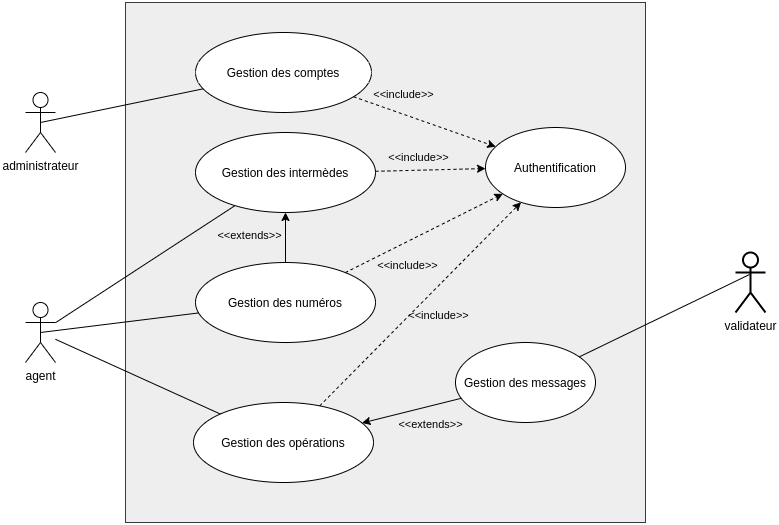
\includegraphics[width=16cm]{chap_2/use-case.png}\cite{}
				\captionof{figure}{Diagramme de cas d'utilisation : vue globle}
				\label{figure9}
			\end{center}
		\subsubsection{Étude détaillée des cas d'utilisation}
		\newpage
		\subsection*{Authentification}
			 \begin{table}[!h]
			 	\begin{center}
			 		\noindent {\renewcommand{\arraystretch}{1.5}\begin{tabularx}{\textwidth}{|l|X|}
			 				\hline & Description \\
			 				\hline Acteur principal & Agent de l'entreprise \\
			 				\hline Objectif & Se connecter pour avoir accès aux différentes fonctionnalités de l'application\\
			 				\hline Pré-conditions & Les informations sur l'agent doivent exister dans la base de données.\\
			 				\hline Déclencheur & Lancement de la page d'authentification\\
			 				\hline
			 				Scénario nominal & Affichage du formulaire de connexion contenant l'email et le mot de passe. 
			 				L'agent renseigne ses identifiants et le système à son tour vérifie l'authenticité de ces informations.\newline
			 				Si ces informations sont correctes alors l'agent est dirigé vers la page d'accueille.
			 				\\
			 				\hline
			 				Extensions &  Si les identifiants envoyés sont incorrectes alors un message d'erreur lui est envoyé. \\ 
			 				\hline               
			 		\end{tabularx}}
			 	\end{center}
			 	\caption{Description de l'authentification} 
			 	\label{Tableau authentification}
			 \end{table}
			 \noindent
		\newpage
		\subsection*{Gestion des comptes}
		Dans cas d'utilisation, il revient à l'administrateur du système de créer les comptes des différents agents du système et leur attribuer un rôle à certaines pages de l'application en fonction de leurs rôles.
			\begin{center}
				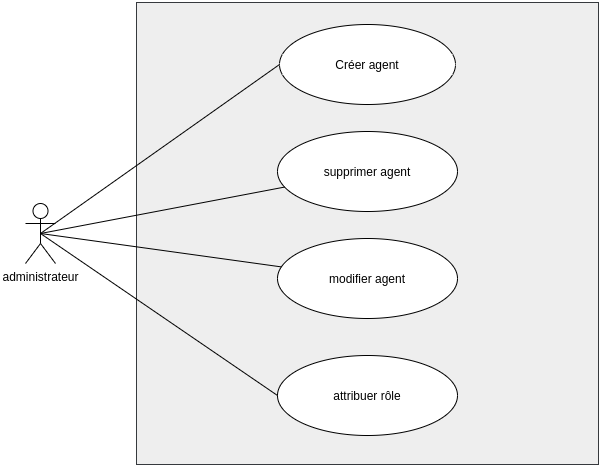
\includegraphics[scale=0.5]{chap_2/gestion-compte.png}
				\captionof{figure}{Diagramme de cas d'utilisation : gestion des comptes}
				\label{cas d'utilisateur gestion compte}
			\end{center}
			\begin{table}[H]
				\begin{center}
					 {\renewcommand{\arraystretch}{1.5}\begin{tabularx}{\textwidth}{|l|X|}
							\hline & Description \\
							\hline Acteur principal & Administrateur\\
							\hline Objectif & Enregistrer les agents de l'entreprise dans la base de donnée et attribuer à chacun d'eux un rôle.\\
							\hline Pré-conditions & Etre authentifier et avoir le rôle \textbf{admin}\\
							\hline Déclencheur & Lancement de la page d'authentification\\
							\hline
							Scénario nominal & Affichage du formulaire de connexion contenant l'email et le mot de passe. 
							L'utilisateur saisit ses identifiants et le système à son tour vérifie l'authenticité de des données entrées.\newline
							Si les informations entrées sont correctes alors l'agent est dirigé vers la page d'administration.
							\\
							\hline
							Extensions &  Si les informations entrées sont incorrectes alors un message d'erreur lui est envoyé. \\
							\hline               
					\end{tabularx}}
				\end{center}
				\caption{Description de cas d'utilisation : Gestion des compte} 
				\label{Table compte}
			\end{table}
		\subsection*{Gestion des intermèdes}
			Dans ce cas d'utilisateur, la tâche revient au personnel agent de gérer tout ce qui concerne les intermèdes.
			\begin{center}
				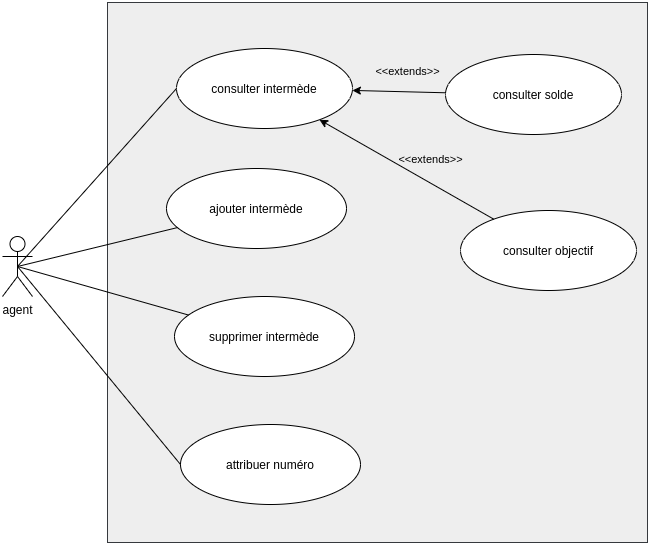
\includegraphics[scale=0.5]{chap_2/use-intermede.png}
				\captionof{figure}{Diagramme de cas d'utilisation : gestion des comptes}
				\label{cas d'utilisateur gestion des intermèdes}
			\end{center}
			\begin{table}[!h]
				\begin{center}
					{\renewcommand{\arraystretch}{1.5}\begin{tabularx}{\textwidth}{|l|X|}
							\hline & Description \\
							\hline Acteur principal & Agent de l'entreprise \\
							\hline Objectif & Avoir la possibilité de gérer la liste des intermèdes dans le but de pouvoir l'étendre, réduire et mettre à jour des informations les concernant .\\
							\hline Pré-conditions & Être authentifié\\
							\hline Description & Une fois l'agent connecté, il a accès aux différentes pages qui lui permettront de gérer les intermèdes
							\\
							\hline              
					\end{tabularx}}
				\end{center}
				\caption{Description du cas d'utilisation: Gestion des intermèdes}
			\end{table}
		\subsection*{Gestion des numéros}
			\begin{table}[H]
				\begin{center}
					{\renewcommand{\arraystretch}{1.5}\begin{tabularx}{\textwidth}{|l|X|}
							\hline & Description \\
							\hline Acteur principal & Agent de l'entreprise \\
							\hline Objectif & Mettre à jour les numéros des intermèdes, créer de nouveaux numéros.\\
							\hline Pré-conditions & Avoir au moins un intermède existant.\\
							\hline Déclencheur & Lancement de la page d'authentification.\\
							\hline
							Scénario nominal &
							Choisir l'intermède.\newline
							Saisir le numéro.\newline
							Attribuer numéro.\newline\newline
							Enregistrer un numéro.\newline
							Mettre à jour numéro.\newline
							Supprimer numéro.\\
							\hline
							Extensions & Si aucun n'intermède n'existe alors il sera impossible d'enregistrer un nouveau numéro. \\ 
							\hline               
					\end{tabularx}}
				\end{center}
				\caption{Description du cas d'utilisateur : Gestion des numéros}
			\end{table}
		\subsection*{Gestion des opérations}
			\begin{center}
				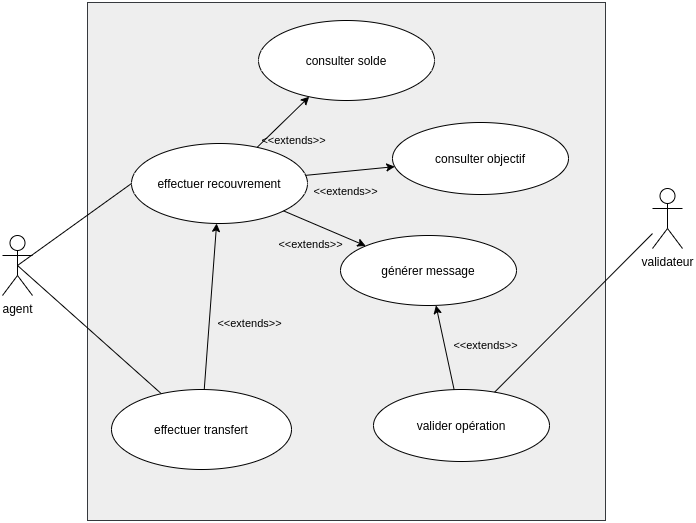
\includegraphics[scale=0.5]{chap_2/gestion-operation.png}
				\captionof{figure}{Diagramme de cas d'utilisation : gestion des opérations}
				\label{Gestion des opérations}
			\end{center}
			\begin{table}[H]
				\begin{center}
					{\renewcommand{\arraystretch}{1.5}\begin{tabularx}{\textwidth}{|l|X|}
							\hline & Description \\
							\hline Acteur principal & Agent de l'entreprise et validateur \\
							\hline Objectif & Effectuer recouvrement(Dépôt ) et transfert d'argent sur les numéros des intermèdes\\
							\hline Pré-conditions & Être authentifié\\
							\hline
							Scénario nominal & Sélectionner le grâce à son code ou son nom.\newline
							Saisir le montant à transférer.\newline\newline
							Choisir le mode de paiement. Si le mode de paiement choisit correspond à un paiement bancaire, alors un nouveau champ apparait pour saisir la référence bancaire. Dans le cas d'un recouvrement ou dépôt tous les modes de paiement de paiement sont autorisés sauf le mode de paiement à crédit.\newline\newline
							Lancer l'opération.\newline\newline
							Un message approuvant le qui l'opération a été effectuée est généré.\newline\newline
							Le validateur récupère le message et valide le opération de manière concrète grâce à la syntaxe appropriée par exemple il effectue:\newline
							*413*NUMERO*MONTANT*00000\# sachant bien que le NUMERO et le MONTANT sont contenus dans le message récupéré.\newline
							Une fois l'opération validée concrètement, le validateur renvoie reçu.\newline
							Impression de la facture.
							\\
							\hline
							Extensions &  Si les informations envoyées sont incorrectes alors un message d'erreur est affiché \\ 
							\hline               
					\end{tabularx}}
				\end{center}
				\caption{Description du cas d'utilisateur : Gestion des opérations}
			\end{table}
		\subsection*{Gestion des messages}
			\begin{center}
				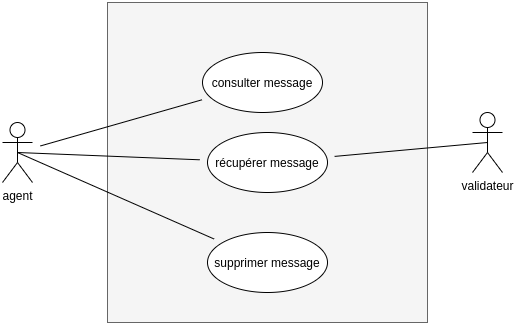
\includegraphics[scale=0.5]{chap_2/message.png}
				\captionof{figure}{Diagramme de cas d'utilisation : gestion des messages}
				\label{Gestion des messages}
			\end{center}
			\begin{table}[H]
				\begin{center}
					{\renewcommand{\arraystretch}{1.5}\begin{tabularx}{\textwidth}{|l|X|}
							\hline & Description \\
							\hline Acteur principal & Agent et validateur \\
							\hline Objectif & Traiter les messages générés après chaque opération.\\
							\hline Pré-conditions & . Être authentifié\\
							\hline Déclencheur & Opération effectuée\\
							\hline
							Scénario nominal & Une fois qu'une opération est effectuée, un  nouveau message est généré avec \textbf{l'état initié}.\newline
							Une fois que le message est récupéré, son état du message passe à l'état '\textbf{en cours d'exécution}'.\newline
							Enfin, lorsque l'opération est finalement validée, alors l'etat du message passe à \textbf{clôturer}
							\\
							\hline              
					\end{tabularx}}
				\end{center}
				\caption{Description de l'authentification} 
			\end{table}
		\subsection{Diagramme de classe}
			\subsubsection{Définition de classe}
				Une classe est un ensemble de données et de fonctions regroupées dans une même entité. Une classe est une description abstraite d'un objet. Les fonctions permettant de manipuler la classe sont appelées méthodes. Instancier une classe consiste à créer un objet sur son modèle.
			\subsubsection{Représentation d'une classe}
				Une classe est représentée par rectangle subdiviser en trois compartiments dans laquelle:
				\begin{itemize}
					\item Le premier compartiment contient le nom de classe
					\item Le deuxième contient la liste des attributs de classe ainsi que leur visibilité (public, protégée ou privée).
					\item Le troisième compartiment représente la liste des méthodes permettant de manipuler les différents attributs de classe.
				\end{itemize}
			En gros une classe se présente comme le montre la figure suivante:
			\begin{center}
				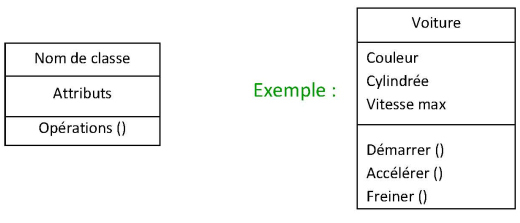
\includegraphics{images/img-1.jpg}\cite{image_classe_voiture}
				\captionof{figure}{représentation d'une classe}
				\label{figure1}
			\end{center}
			\subsubsection{Les attributs}
				Les attributs représentent les données qui caractérisent l'objet. Les attributs sont aussi définis par leurs types (entier, chaîne de caractère, caractère, etc. ).
			\subsubsection{Les méthodes}
				Les méthodes d'un objet caractérisent son comportement, c'est-à-dire l'ensemble des actions (appelées opérations) que l'objet est à même de réaliser.
			\subsubsection{Notion de multiplicité}
				La multiplicité définit le nombre d'instances de l'association pour une instance de la classe\cite{}.
				La multiplicité est définie par un nombre entier ou un intervalle de valeurs, elle est aussi la traduction d'une règle de gestion.
				\begin{center}
					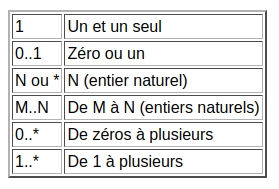
\includegraphics{images/img-2.png}
					\captionof{figure}{multiplicité}
					\label{figure2}
				\end{center}
			\subsubsection{Les associations}
			Les associations permettent de préciser les relations qui peuvent exister entre deux ou plusieurs objets.
			L'association se fait entre classe et non entre les instances. Lorsque une association est
			définie entre deux classes, cela signifie que les objets instances de ces deux classes
			peuvent être reliés entre eux.
			\begin{center}
				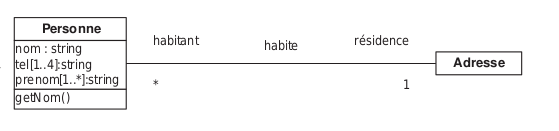
\includegraphics[width=\columnwidth]{images/assoc-1.png}
				\captionof{figure}{association}
				\label{figure3}
			\end{center}
		\subsubsection{implémentation}
		Identification des classes:\\
		
		\textbf{Personnel}(ID:integer, nom:string, prenom:string, email)\\
		
		\textbf{Intermed}(ID:integer, code:string, nom:string, solde:integer)\\
		
		\textbf{Numero}(ID:integer, numero:string)\\
		
		\textbf{Objectif}(ID:integer, mois:string, objectif:integer, bilan:integer)\\
		
		\textbf{Operation}(ID:integer, montant:integer, reference:string, date)\\
		
		\textbf{Transfert}(ID:integer, numero:string)\\
		
		\textbf{Secteur}(ID:integer, nom:string)\\
		
		\textbf{Agence}(ID:integer, nom:string)\\
		
		\textbf{Statut}(ID:integer, nom:string)\\
		
		\textbf{Etat}(ID:integer, nom:string, commentaire:text)\\
		
		\textbf{Message}(ID:integer, sms:text, date:Date)\\
		
		\textbf{Facture}(ID:integer, numeroFac:string, date:Date)\\
		
		\textbf{Mode de paiement}(ID:integer, nom:string)\\
		
		\textbf{Ouverture}(ID:integer, jour:string, code:string)\\
		
		\begin{center}
			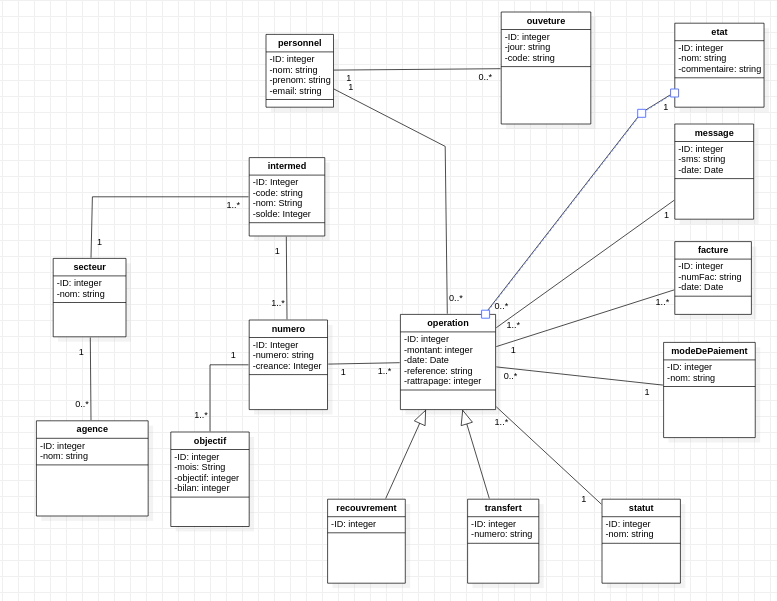
\includegraphics[width=16cm]{images/diagramme.png}
			\captionof{figure}{diagramme de classe de l'application}
		\end{center}
	
	\subsubsection{Description des classe}
	
		\begin{tabular}{|l|l|l|l|}
			\hline
			\multicolumn{4}{|c|}{\textbf{Classe Peronnel : représente les effectuant les opérations}}\\
			\hline
			
			 & \textbf{Nom} & \textbf{Description} & \textbf{Type} \\
			\multirow{4}{*}{Attributs} & ID & code permettant d'identifié le personnel & Numérique \\
			& nom & désigne le nom personnel & chaîne de caractère \\
			& prénom & désigne le prénom de personnel & chaîne de caractère \\
			& email & addresse électronique de l'intermed & chaîne de caractère\\
			\hline
		\end{tabular}
		\captionof{table}{tableau de classe \textit{Personnel}}
		\label{table1}
		
		\begin{tabular}{|l|l|l|l|}
			\hline
			\multicolumn{4}{|c|}{\textbf{Classe Intermed : représente les effectuant les opérations}} \\
			
			\hline
			
			& \textbf{Nom} & \textbf{Description} & \textbf{Type} \\
			\multirow{3}{*}{Attributs} & ID & code permettant d'identifié l'intermed & numérique \\
			
			& code & code unique permettant d'identifier l'intermed &  chaîne de caractère \\
			
			& nom & désigne le nom l'intermède & chaîne de caractère \\
			
			& solde & désigne le solde l'intermède & numérique \\
			\hline
		\end{tabular}
		\captionof{table}{tableau de classe Intermed}
		\label{table2}
		
		\begin{tabular}{|l|l|l|l|}
			\hline
			\multicolumn{4}{|c|}{\textbf{Classe Numéro : numéro appartenant à un intermède}} \\
			
			\hline
			
			& \textbf{Nom} & \textbf{Description} & \textbf{Type} \\
			\multirow{3}{*}{Attributs} & ID & permet d'identifier le numéro & numérique \\
			
			& numéro & numéro de l'intermède & chaîne de caractère \\
			
			& créance & créance de l'intermède sur ce numéro  & numérique \\
			
			\hline
			
		\end{tabular}
		\captionof{table}{tableau de classe \textit{Numéro}}
		\label{table3}
		
		\begin{tabular}{|l|l|l|l|}
			\hline
			\multicolumn{4}{|c|}{\textbf{Classe Objectif : représente les effectuant les opérations}} \\
			
			\hline
			
			& \textbf{Nom} & \textbf{Description} & \textbf{Type} \\
			\multirow{3}{*}{Attributs} & ID & identifiant de l'objectif d'un numéro & numérique \\
			
			& mois & mois dans lequel l'objectif à été effectué &  chaîne de caractère \\
			
			& objectif & objectif du numéro &chaîne de caractère \\
			
			& bilan & bilan de l'objectif & numérique \\
			
			\hline
			
		\end{tabular}
		\captionof{table}{tableau de classe \textit{objectif}}
		\label{table4}
		
		
		\begin{tabular}{|l|l|l|l|}
			\hline
			\multicolumn{4}{|c|}{\textbf{Classe Opération: désigne les opérations pouvant être par le personnel}} \\
			
			\hline
			
			& \textbf{Nom} & \textbf{Description} & \textbf{Type} \\
			\multirow{3}{*}{Attributs} & ID & identifiant de l'opération & numérique \\
			
			& montant & montant à transféré ou à déposer & numérique\\
			
			& date & date à laquelle l'opération s'est effectuée & numérique \\
			
			& référence & chaîne de caractère pouvant identifier l'opération & chaîne de caractère\\
			
			& rattrapage & entier permettant de spécifier si l'opération s'est bien déroulée & entier \\
			
			\hline
			
		\end{tabular}
		\captionof{table}{tableau de classe \textit{Opération}}
		\label{table5}
		
		\begin{tabular}{|l|l|l|l|}
			\hline
			\multicolumn{4}{|c|}{\textbf{Classe Etat : définie l'ensemble des statut que peux pendre une opération}} \\
			
			\hline
			
			& \textbf{Nom} & \textbf{Description} & \textbf{Type} \\
			\multirow{3}{*}{Attributs} & ID & code permettant d'identifié l'intermed & numérique \\
			
			& nom & nom du statut qui peut prendre les valeurs suivantes: \textit{initié}, \textit{en cours d'exécution}, \textit{exécuté}, \textit{annulé} et \textit{supprimé}\\
			
			\hline
			
		\end{tabular}
		\captionof{table}{tableau de classe \textit{Etat}}
		\label{table6}
		
		\begin{tabular}{|l|l|l|l|}
			\hline
			\multicolumn{4}{|c|}{\textbf{Classe Message : message de transfert après qu'une opération ait été effectuée}} \\
			
			\hline
			
			& \textbf{Nom} & \textbf{Description} & \textbf{Type} \\
			\multirow{3}{*}{Attributs} & ID & identifiant du message & numérique \\
			
			& sms & message de transfert &  texte\\
			
			& date & date à laquelle le message a été reçu & date \\
			
			\hline
			
		\end{tabular}
		\captionof{table}{tableau de classe \textit{message}}
		\label{table7}
		
		\begin{tabular}{|l|l|l|l|}
			\hline
			\multicolumn{4}{|c|}{\textbf{Classe transfert : classe fille de la classe opération spécialisée dans le transfert}} \\
			
			\hline
			
			& \textbf{Nom} & \textbf{Description} & \textbf{Type} \\
			\multirow{3}{*}{Attributs} & ID & permet d'identifier le transfert effectué & numérique \\
			
			& numéro & numéro sur lequel le transfert sera effectué & chaîne de caractère\\
			
			\hline
			
		\end{tabular}
		\captionof{table}{tableau de classe \textit{transfert}}
		\label{table15}
		
		
		\begin{tabular}{|l|l|l|l|}
			\hline
			\multicolumn{4}{|c|}{\textbf{Classe recouvrement : classe fille de la classe \textit{opération} spécialisée dans le recouvrement}} \\
			
			\hline
			
			& \textbf{Nom} & \textbf{Description} & \textbf{Type} \\
			\multirow{1}{*}{Attributs} & ID & permet d'identifier le recouvrement effectué & numérique \\
			\hline
			
		\end{tabular}
		\captionof{table}{tableau de classe \textit{recouvrement}}
		\label{table16}
		
		\begin{tabular}{|l|l|l|l|}
			\hline
			\multicolumn{4}{|c|}{\textbf{Classe Facture : facture délivrée après une opération}} \\
			\hline
			
			& \textbf{Nom} & \textbf{Description} & \textbf{Type} \\
			\multirow{3}{*}{Attributs} & ID & identifiant permettant de retrouver la facture & numérique \\
			
			& numFac & numéro unique permettant d'identifier la facture &  chaîne de caractère \\
			
			& date & date à laquelle la facture a été délivrée & chaîne de caractère \\
			
			\hline
			
		\end{tabular}
		\captionof{table}{tableau de classe \textit{facture}}
		\label{table8}
		
		
		\begin{tabular}{|l|l|l|l|}
			\hline
			\multicolumn{4}{|c|}{\textbf{Classe ModePaiement : représente les effectuant les opérations}} \\
			
			\hline
			
			& \textbf{Nom} & \textbf{Description} & \textbf{Type} \\
			\multirow{3}{*}{Attributs} & ID & identifiant unique attribué à un mode paiement  & numérique \\
			
			& nom & nom du mode de paiement &  chaîne de caractère \\
			
			\hline
			
		\end{tabular}
		\captionof{table}{tableau de classe \textit{ModePaiement}}
		\label{table9}
		
		
		\begin{tabular}{|l|l|l|l|}
			\hline
			\multicolumn{4}{|c|}{\textbf{Classe ouverture : représente les effectuant les opérations}} \\
			
			\hline
			
			& \textbf{Nom} & \textbf{Description} & \textbf{Type} \\
			\multirow{3}{*}{Attributs} & ID & identifiant des jours d'ouverture & numérique \\
			
			& jour & jour d'ouverture & chaîne de caractère \\
			
			& code & code d'ouverture & chaîne de caractère \\
			\hline
			
		\end{tabular}
		\captionof{table}{tableau de classe \textit{ouverture}}
		\label{table10}
		
		
		\begin{tabular}{|l|l|l|l|}
			\hline
			\multicolumn{4}{|c|}{\textbf{Classe agence : définie l'agence}} \\
			
			\hline
			
			& \textbf{Nom} & \textbf{Description} & \textbf{Type} \\
			\multirow{3}{*}{Attributs} & ID & identifiant permettant d'identifier l'agence & numérique \\
			
			& nom & désigne le nom de l'agence& chaîne de caractère \\
			
			\hline
			
		\end{tabular}
		\captionof{table}{tableau de classe \textit{agence}}
		\label{table14}
		
		
		\begin{tabular}{|l|l|l|l|}
			\hline
			\multicolumn{4}{|c|}{\textbf{Classe Secteur : secteur au lequel appartient l'agence}} \\
			
			\hline
			
			& \textbf{Nom} & \textbf{Description} & \textbf{Type} \\
			\multirow{3}{*}{Attributs} & ID & identifiant du secteur & numérique \\
			
			& nom & nom du secteur &  chaîne de caractère \\
			
			\hline
			
		\end{tabular}
		\captionof{table}{tableau de classe \textit{secteur}}
		\label{table11}
		
		\section{Schéma relationnel}
			\subsection{Modèle logique des données ou MLD}
				\subsubsection{Définition}
					Le modèle logique des données consiste à décrire la structure de données utilisée sans faire référence à un langage de programmation. Il s'agit donc de préciser le type de données utilisées lors des traitements. Ainsi, le modèle logique est dépendant du type de base de données utilisé.
				\subsubsection{Liste des tables}
					
					\textbf{PERSONNEL}(\underline{\textbf{ID}}, nom, prenom, email)\\
					
					\textbf{SECTEUR}(\underline{\textbf{ID}}, nom)\\
					
					\textbf{AGENCE}(\underline{\textbf{ID}}, \#secteur\_id, nom)\\
					
					\textbf{INTERMED}(\underline{\textbf{ID}}, code, nom, solde)\\
					
					
					\textbf{NUMERO}(\underline{\textbf{ID}}, \#intermed\_id, numero, creance)\\
					
					\textbf{objectif}(\underline{\textbf{ID}}, \#numero\_id, mois, objectif, bilan)\\
					
					\textbf{MODEDEPAIEMENT}(\underline{\textbf{ID}}, nom)\\
					
					\textbf{STATUT}(\underline{\textbf{ID}}, nom)\\
					
					\textbf{ETAT}(\underline{\textbf{ID}}, nom)\\
					
					\textbf{OPERATION}(\underline{\textbf{ID}}, \#personnel\_id, \#numero\_id, \#modepaiement\_id, \#statut\_id, \#etat\_id, montant, date, reference, rattrapage)\\
					
					\textbf{OUVERTURE}(\underline{\textbf{ID}}, \#personnel\_id, jour, code)\\
					
					\textbf{TRANSFERT}(\underline{\textbf{ID}},\#personnel\_id, \#numero\_id, \#modepaiement\_id, \#statut\_id, \#etat\_id, rattrapage, montant, reference, date)\\
					
					\textbf{RECOUVREMENT}(\underline{\textbf{ID}},\#personnel\_id, \#modepaiement\_id, \#statut\_id, \#etat\_id, rattrapage, montant, reference, date)\\
					
					\textbf{FACTURE}(\underline{\textbf{ID}}, \#operation\_id, numFac, date)\\
					
					\textbf{MESSAGE}(\underline{\textbf{ID}}, \#operation\_id, sms, date)\\
			\subsection{Modèle physique de donnée ou MPD}
			
				\subsubsection{Définition}
					Un modèle de données physique est un modèle spécifique à une base de données, qui représente des objets de données relationnelles (par exemple, tables, colonnes, clés principales et externes) et leurs relations.
				\subsubsection{Représentation du MPD}
					\includegraphics[width=\columnwidth]{images/database.png}
					\captionof{figure}{Modèle physique des données}
					\label{modèle physique des données}
	\section{Outils de développement}
		\subsection{Technologie front-end}
			\subsubsection{HTML 5}
				L'HyperText Markup Language, HTML, désigne un type de langage informatique descriptif. Il s'agit plus précisément d'un format de données utilisé dans l'univers d'Internet pour la mise en forme des pages Web. Il permet, entre autres, d'écrire de l'hypertexte, mais aussi d'introduire des ressources multimédias dans un contenu.\\
				
				Développé par le W3C (World Wide Web Consortium) et le WHATWG (Web Hypertext Application Technology Working Group), le format ou langage HTML est apparu dans les années 1990. Il a progressivement subi des modifications et propose depuis 2014 une version HTML5 plus aboutie.\\
				
				L'HTML est ce qui permet à un créateur de sites Web de gérer la manière dont le contenu de ses pages Web va s'afficher sur un écran, via le navigateur.\cite{definition_html}
				
				\begin{center}
					
\includegraphics[width=2cm]{chap_2/html5.png}
					\captionof{figure}{Logo HTML 5}
					\label{figure5}
				\end{center}
			
			\subsubsection{CSS 3}
			
			Les feuilles de styles (en anglais "Cascading Style Sheets", abrégé CSS) sont un langage qui permet de gérer la présentation d'une page Web. Le langage CSS est une recommandation du World Wide Web Consortium (W3C), au même titre que HTML ou XML. Aujourd'hui nous sommes à la version 3 d'où CSS 3.
				
				\begin{center}
					
\includegraphics[width=2cm]{chap_2/css3.png}
					\captionof{figure}{Logo CSS 3}
					\label{figure6}
				\end{center}
			
			\subsubsection{Bibliothèque CSS - Bootstrap 5}
				
				Bootstrap est une bibliothèque CSS permettant de donner une apparence sublime aux sites web.L'une de ces forces est son côté responsive qui permet au site de s'adapter sur les grands et petits écrans (mobile)
				
				\begin{center}
					
\includegraphics[width=5cm]{chap_2/bootstrap.png}
					\captionof{figure}{Logo Bootstrap 5}
					\label{figure7}
					\cite{logo_bootstrap}
				\end{center}
			
			\subsubsection{Bibliothèque  JavaScript - AlpineJS}
			
			Alpine est un outil robuste et minimal pour composer des comportements directement dans notre code HTML. Il apporte une réactive flexible comme d'autre bibliothèque JS (React par exemple).\\
		
			\begin{center}
				
\includegraphics[width=10cm]{chap_2/alpine.png}
				\captionof{figure}{Logo AlpineJS}
				\label{figure8}
				\cite{logo_alpine}
			\end{center}
				
		\subsection{Choix du framework back-end}
			\section*{Laravel}
				\begin{center}
					
\includegraphics[scale=0.2]{chap_2/laravel.png}
					\captionof{figure}{Logo de Laravel}
					\label{logo de laravel}
					\cite{logo_laravel}
				\end{center}
			Dans cette application, nous avons décidé de nous tourner vers l'un des framework PHP le plus populaire et le plus utilisé : \textbf{Laravel}.\newline
			En effet Laravel est le framework PHP open source le mieux noté sur GitHub. Fondé en 2011 par Taylor Otwell, Laravel utilise le pattern MVC et est orienté objet.\cite{laravel_1}\newline
			Que de réinventer la roue, Laravel se base sur des technologies existantes.\\
			Laravel se base sur \textbf{Symfony} pour créer son système de routage. De même pour l'envoie des mails Laravel utilise la bibliothèque \textbf{SwiftMailer}.
			\subsection*{Avantage}
				\begin{itemize}
					\item[$\bullet$] Il est facile à installer et présent chez tous les hébergeurs.
					\item[$\bullet$] Basé sur l'architecture MVC(Model View Controller)qui donne une meilleure organisation au niveau du code et avec une hiérarchie de dossiers très bien fait.
					\item[$\bullet$] Grande communauté et beaucoup de documentation
					\item[$\bullet$] Possibilité de faire tests unitaires afin de garantir qu’il n’y a pas de bogues ou d’exceptions l'application
					\item[$\bullet$] Développement plus rapide grâce aux helpers déjà disponible.
				\end{itemize}
			\section*{Livewire}
				\begin{center}
					
\includegraphics[scale=0.6]{chap_2/livewire.png}
					\captionof{figure}{Logo de Livewire}
					\label{logo de livewire}
					\cite{logo_livewire}
				\end{center}
				\subsection*{Présentation}
					Livewire est un package Laravel, qui aux permet développeur Laravel de créer des applications Web réactives en utilisant Laravel Blade comme langage de templating sans écrit la moindre ligne de code.
					
				\subsection*{Avantages}
				\begin{itemize}
					\item[$\bullet$] Créer des application réactive en restant dans le confort Laravel sans écrit la moindre ligne de code JavaScript.
					\item[$\bullet$] Crée facilement des composants réutilisables
					\item[$\bullet$] Plusieurs fonctions (ou encore \textbf{helper}) disponible pour rendre encore plus facile sa prise en main.
				\end{itemize}
			
			
		\subsection{Système de gestion de base de données}
		\newpage
			\section*{MySQL}
			\begin{center}
				
\includegraphics[scale=0.2]{chap_2/mysql.png}
				\captionof{figure}{Logo de MySQL}
				\label{logo de MySQL}
				\cite{logo_mysql}
			\end{center}
			Et surtout MySQL, qui est un Système de Gestion de Bases de Données Relationnelles (abrégé SGBDR), c'est-à-dire un logiciel qui permet de gérer des bases de données, et donc de gérer de grosses quantités d'informations. Il utilise pour cela le langage SQL. Il s'agit d'un des SGBDR les plus connus et les plus utilisés.
			\subsection{Avantages}
				\begin{itemize}
					\item[$\bullet$] Grâce à sa popularité, MySQL dispose d'une grande communauté, ce qui implique qu'on peut facilement trouver de l'aide en cas de difficulté.
					\item[$\bullet$] il est totalement open source et gratuit.
					\item[$\bullet$] il est en plus multi-threadé et multi-utilisateurs.
					\item[$\bullet$] Ses performances sont excellentes
				\end{itemize}
			
		\subsection{Architecture structurel}
		\subsection*{MVC}
			Modèle-vue-contrôleur ou MVC est un motif d'architecture logicielle destiné aux interfaces graphiques lancé en 1978 et très populaire pour les applications web. Le motif est composé de trois types de modules ayant trois responsabilités différentes : les modèles, les vues et les contrôleurs.
				
				\begin{center}
					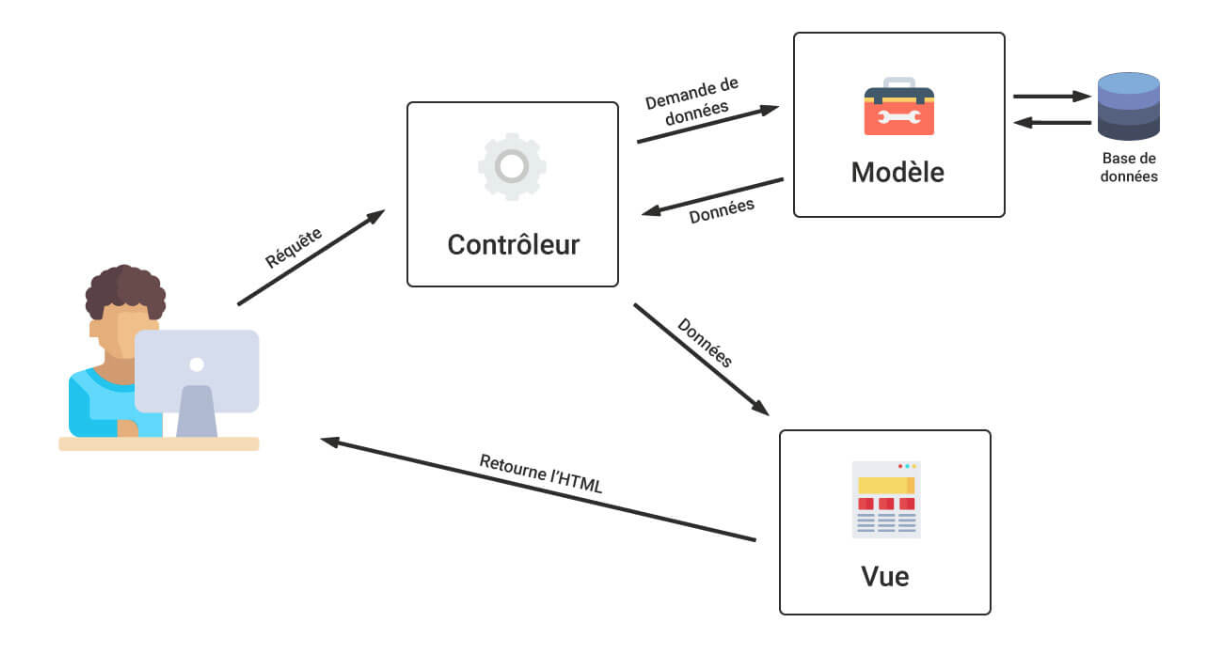
\includegraphics[scale=0.5]{chap_2/mvc.png}
					\captionof{figure}{MVC}
					\label{logo de MVC}
					\cite{logo_mvc}
				\end{center}
				
			\subsubsection{Model}
				cette partie gère les données de l'application. Son rôle est d'aller récupérer les informations « brutes » dans la base de données, de les organiser et de les assembler pour qu'elles puissent ensuite être traitées par le contrôleur. On y trouve donc entre autres les requêtes SQL\cite{mvc_model}. Dans une application laravel le Model est géré par Eloquent qui est Object Relationnal Mapping.
			\subsubsection{View}
				 Cette partie se concentre sur l'affichage. Elle ne fait presque aucun calcul et se contente de récupérer des variables pour savoir ce qu'elle doit afficher. On y trouve essentiellement du code HTML mais aussi quelques boucles et conditions PHP très simples.
			\subsubsection{Controller}
				Cette partie gère la logique du code qui prend des décisions. C'est en quelque sorte l'intermédiaire entre le modèle et la vue : le contrôleur va demander au modèle les données, les analyser, prendre des décisions et renvoyer le texte à afficher à la vue.
		\subsection{Autre outils utilisés}
			\subsection*{Mysql Workbench}
				\begin{center}
					
\includegraphics[scale=0.5]{chap_2/workbench.jpeg}
					\captionof{figure}{MVC}
					\label{Mysql Workbench}
					\cite{logo_workbench}
				\end{center}
				MySQL Workbench est un logiciel de gestion et d'administration de bases de données MySQL.
			\subsection*{Draw.io}
				\begin{center}
					
\includegraphics[scale=2]{chap_2/drawio.png}
					\captionof{figure}{Draw.io}
					\label{Draw.io}
					\cite{logo_drawio}
				\end{center}
			Draw.io est une application gratuite en ligne, accessible via son navigateur (protocole https) qui permet de dessiner des diagrammes ou des organigrammes. Cet outil vous propose de concevoir toutes sortes de diagrammes, de dessins vectoriels, de les enregistrer au format XML puis de les exporter.\cite{draw_definition}
	\chapter{Choix technologiques}
	\section{Technologie back-end}
		\subsection{Symfony}
			\begin{center}
				
\includegraphics[scale=0.3]{chap_2/symfony.png}
				\captionof{figure}{Symfony}
				\label{Symfony}
			\end{center}
			Symfony est un framework de développement web open-source écrit en PHP. Il fournit un ensemble de composants modulaires et d'outils qui facilitent la création et la maintenance d'applications web complexes et évolutives. Symfony suit les principes de conception du modèle MVC (Modèle-Vue-Contrôleur), ce qui favorise la séparation des préoccupations et la structuration claire du code.\\
			Les caractéristiques principales de Symfony incluent :
			\begin{itemize}
				\item \textbf{Composants réutilisables} : Symfony est basé sur un ensemble de composants indépendants, tels que le gestionnaire de dépendances, le système de routage, le composant de formulaire, le composant de sécurité, etc. Ces composants peuvent être utilisés de manière modulaire dans différentes applications.
				\item \textbf{Productivité} : Symfony propose des outils et des générateurs de code qui accélèrent le développement. Il offre également une interface en ligne de commande (CLI) pour effectuer des tâches courantes telles que la génération de code, la gestion de bases de données et les tests.
				\item \textbf{Flexibilité} : Les développeurs peuvent personnaliser et configurer les composants selon les besoins spécifiques de leur projet. Symfony permet également l'intégration de bundles tiers pour ajouter des fonctionnalités supplémentaires.
				\item \textbf{Qualité du code} : Symfony encourage les bonnes pratiques de codage, le test unitaire et fournit des outils pour garantir la qualité du code. Cela facilite la maintenance à long terme des applications.
				\item \textbf{Sécurité} : Symfony offre des fonctionnalités de sécurité intégrées, telles que la gestion des autorisations, la protection contre les vulnérabilités courantes et la prévention des attaques.
				\item \textbf{Documentation} : Symfony dispose d'une documentation complète et détaillée, ainsi que d'une communauté active qui partage des ressources et des solutions aux problèmes courants.
				\item \textbf{Support à long terme} : Symfony suit des cycles de maintenance à long terme, ce qui garantit que les applications développées avec ce framework restent à jour et sécurisées.\\
			\end{itemize}
		
		Symfony est largement utilisé pour développer des applications web de toutes tailles, des sites web simples aux applications d'entreprise complexes. De nombreuses entreprises et projets renommés utilisent Symfony pour sa fiabilité, sa robustesse et sa capacité à accélérer le développement tout en maintenant des normes élevées de qualité et de sécurité.
		
		\subsection{PHPQA}
			\begin{center}
				
\includegraphics[scale=0.3]{chap_3/phpqa.png}
				\captionof{figure}{PHPQA}
				\label{PHPQA}
				\cite{phpqa_image}
			\end{center}
		
		PHPQA est un ensemble d'outils et de techniques destinés à l'analyse statique et dynamique du code PHP, ainsi qu'à l'amélioration de sa qualité et de sa performance. Il vise à aider les développeurs à identifier les problèmes potentiels dans le code, à maintenir de bonnes pratiques de développement et à optimiser les performances de leurs applications.
		
		Les principales catégories d'outils et de pratiques incluses dans PHPQA sont les suivantes :
		\begin{itemize}
			\item \textbf{Analyse statique du code} : Ces outils examinent le code source PHP sans l'exécuter et identifient des erreurs de syntaxe, des problèmes de sécurité, des antipatterns (mauvaises pratiques) et d'autres problèmes potentiels. Des exemples d'outils d'analyse statique populaires sont \textbf{PHPStan}, et \textbf{PHP CodeSniffe}r.
			\item \textbf{Mesure de la couverture de code} : Ces outils mesurent quelle partie du code est couverte par les tests automatisés, aidant ainsi à identifier les zones non testées et à garantir une meilleure couverture.
			\item \textbf{Profiler et analyseurs de performances} : Ces outils permettent de surveiller et d'analyser les performances de l'application en identifiant les goulots d'étranglement, les requêtes lentes et d'autres problèmes de performance. Des outils populaires incluent Xdebug et Blackfire.
			\item \textbf{Documentation du code} : La documentation claire et précise du code est importante pour la compréhension et la maintenance du projet. Des outils comme \textbf{PHPDocumentor} aident à générer une documentation automatique à partir des commentaires du code source.
			\item \textbf{Amélioration du style de code} : Les outils comme \textbf{PHP CS} Fixer aident à maintenir un style de code cohérent en automatisant la correction des espaces, des indentations et d'autres conventions de codage.
		\end{itemize}
		
		En utilisant PHPQA, les développeurs peuvent identifier rapidement les problèmes potentiels dans leur code, améliorer sa qualité, accélérer le processus de développement et optimiser les performances de leurs applications PHP. Cela contribue à créer des applications plus robustes, fiables et performantes.
		
		
		\subsection{Codeception}
			\begin{center}
				
\includegraphics[scale=1]{chap_3/codeception.png}
				\captionof{figure}{Codeception}
				\label{Codeception}
				\cite{codeception_image}
			\end{center}
		Basé sur PHPUnit, Codeception est un framework de test automatisé pour les applications web. Il est principalement utilisé pour effectuer des tests unitaires, fonctionnels et d'acceptation dans le contexte du développement web. Codeception simplifie la création et l'exécution de tests automatisés en fournissant des fonctionnalités spécifiques pour l'émulation d'actions utilisateur, la validation du comportement de l'application.\\
		Aussi, il rassemble et partage les meilleures pratiques et solutions pour tester les applications web PHP. Grâce à un ensemble flexible de modules inclus, les tests sont faciles à écrire, à utiliser et à maintenir \cite{codeception}.\\
		En plus d'offrir les fonctionnalités de PHPUnit, codeception offre de modules intéressants permettant de faire facilement des tests d'acceptance et fonctionnels.
		
		\subsubsection{Docker}
			\begin{center}
				
\includegraphics[scale=1]{chap_3/docker.jpg}
				\captionof{figure}{Docker}
				\label{Docker}
				\cite{docker_image}
			\end{center}
		Docker est une plate-forme open-source qui permet de développer, déployer et exécuter des applications dans des conteneurs légers et portables. Les conteneurs sont des environnements logiciels isolés qui incluent tout ce dont une application a besoin pour s'exécuter, y compris le code, les bibliothèques, les dépendances et les configurations.\\
		Docker permet aux développeurs d'être sur la même longueur d'onde en terme de version de logiciels utilisées lors de la phase de développement. Ce qui peut être très utile pour éviter de potentiels problèmes lors du déploiements d'une application.
		
		
		\subsection{MariaDB}
			\begin{center}
				
\includegraphics[scale=0.5]{chap_3/mariadb.png}
				\captionof{figure}{Docker}
				\label{MariaDB}
				\cite{mariaDB_image}
			\end{center}
		MariaDB est un système de gestion de base de données open-source et relationnel (SGBDR) qui est conçu pour être une alternative compatible avec MySQL. Il a été créé par certains des développeurs originaux de MySQL en réponse à des préoccupations concernant la direction et la gouvernance de MySQL après son acquisition par Oracle Corporation.\\
		MariaDB partage une grande partie de la syntaxe et des fonctionnalités avec MySQL, ce qui signifie que les applications écrites pour MySQL peuvent généralement être utilisées avec MariaDB sans modifications majeures. Cependant, MariaDB propose également des améliorations et des fonctionnalités spécifiques qui en font une option attrayante pour de nombreux utilisateurs.\\
		Les avantages principaux qu'on peut tirer de MariaDB sont:
		\begin{itemize}
			\item \textbf{Performance} : MariaDB inclut des optimisations et des améliorations de performances par rapport à MySQL, notamment dans les domaines de la vitesse d'exécution des requêtes et de la gestion de la mémoire.\cite{chatgpt}
			\item \textbf{Stockage} : MariaDB prend en charge divers moteurs de stockage, y compris InnoDB (le moteur de stockage par défaut), Aria, MyISAM et d'autres.\cite{chatgpt}
			\item \textbf{Haute disponibilité} : MariaDB propose des fonctionnalités de réplication et de clustering pour garantir une haute disponibilité des données et une tolérance aux pannes, etc.\cite{chatgpt}
		\end{itemize}
	
	\section{Technologie back-end}
		\subsection{AdminLTE}
			\begin{center}
				
\includegraphics[scale=0.7]{chap_3/adminlte.png}
				\captionof{figure}{AdminLTE}
				\label{AdminLTE}
				\cite{adminlte_image}
			\end{center}
		AdminLTE est un template open-source de conception d'interface utilisateur (UI) et d'administration pour les applications web. Il fournit une collection de composants, de styles CSS et de scripts JavaScript préconstruits pour créer rapidement des interfaces d'administration élégantes et conviviales.\\
		L'avantage avec Admin Lte, c'est qu'il permet aux développeurs avoir d'un gain de temps énorme et de se concentrer sur la logique métier de l'application, du fait des composants réutilisables mis à leur disposition.
		
		\subsection{ChartJS}
			\begin{center}
				
\includegraphics[scale=0.5]{chap_3/chartjs.png}
				\captionof{figure}{ChartJS}
				\label{ChartJS}
				\cite{chartjs_image}
			\end{center}
			ChartJS est une bibliothèque JavaScript open source gratuite pour la visualisation de données. Créée par le développeur web Nick Downie en 2013, la bibliothèque est maintenant maintenue par la communauté et est la deuxième bibliothèque de graphiques JS la plus populaire sur GitHub par le nombre d'étoiles après D3.js. Chart.js est rendu dans un canvas HTML5. Elle est disponible sous la licence MIT.\cite{chartjs}\\
			Pour réaliser les diagrammes d'évolutions et les courbes de tendance, ChartJS a été un élement essentiel, voir indispensable.
			
		\subsection{ReactJS}
			\begin{center}
				
\includegraphics[scale=0.4]{chap_3/react.png}
				\captionof{figure}{React}
				\label{ReactJS}
				\cite{react_js}
			\end{center}
			React JS est une biblithèque javascript développée par Facebeook depuis 2013 \cite{react_wiki}. Il offre la de possibilité de créer des composants réactive grâce aux hooks. React a pour avantage d'être utilisé en fonction de l'état d'un projet (from scratch ou en plein milieu). Pour un projet demarré à partir de zéro, il est possible de créer une application full-react, dont la mise en place est juste éffectuée par une commande (\textbf{create-react-app}).\\
			Dans le cas de notre application il a été utilisé (grâce à Symfony UX) pour rendre le tableau des bluids plus réactif à chaque clique d'un utilisateur.	
	\chapter*{Conclusion générale}

	Dans le monde du développement informatique, pour mettre en place une application qui puisse être maintenable, il est important de suivre un chemin logique qui part de la conception jusqu'au choix des outils techniques pour la réalisation du projet.\\	C'est à partir de ce raisonnement que nous nous sommes posés de nombreuses questions quant au choix de la méthode de modélisation, de l'outil de développement, etc, pour mener à bien la réalisation de ce projet.
	Ce projet a été inspiré d'une application legacy (une vielle application) qui ne pouvait plus être maintenue par le fait de la non disponibilité de son code source et aussi de l'architecture sur laquelle elle reposait. C'est à partir de ce fait, que nous nous sommes fixés comme objectif de fournir une application qui bien évidemment basée sur une architecture simple pourra s'adapter aux besoins de l'entreprise et fournir plus de fonctionnalités dans le but de faciliter les différentes activités menées au sein de l'entreprise ONEMART.\\
	
	La réalisation de cette application nous a été bénéfique sur plusieurs points. Elle nous a permis de comprendre le sens réel de la pratique dans le domaine informatique car grâce à la pratique, nous avons touché à tout ce qui est API Rest, faire le tour du développement WEB et sans oublier la structuration de code que nous avons tirée de l'architecture MVC.\\
	
	En réalité, en partant de la conception jusqu'à la réalisation , le développement de cette application nous a également permis de nous perfectionner en améliorant nos connaissances en programmation informatique et en conception.Il aussi important de noter que grâce à ce projet, nous avons compris et mis en œuvre le déroulement d'un cycle de vie d'un logiciel.\\
	
	A l'issue de notre stage, nous d'autres idées d'amélioration nous sont venues en tête qui consiste à la mise en application d'une application mobile pour chaque agent l'entreprise.\\
	C'est ainsi que nous nous posés la question principale suivante :\\
	
	A l'aide des points d'entrées définies, comment mettre en place une application mobile pouvant effectuer les opérations de rechargements et transferts sans disposée de la puce e-master ?
	
	\addcontentsline{toc}{chapter}{webographiques}
\bibliography{bibliographie/bibliographie}
\bibliographystyle{unsrt}
	
\end {document}